% File: dist-css-c305.tex
% CSS lattice for .tex

\documentclass{standalone}

% preamble for jupiter-paper related TikZ drawing
\usepackage{tikz}
\usetikzlibrary{shapes, positioning, arrows.meta, calc, backgrounds, fit}

% default horizontal/vertical distance
\def\hdist{1.5}
\def\vdist{1.5}

\newcommand{\state}[2]{% #1: state label; #2: position
  \node (#1) [circle, inner sep = 0pt, minimum size = 10mm, text width = 10mm, align = center, draw, #2, font = \Large] {$#1$};
}

\newcommand{\transition}[4][]{% #2: start state; #3: end state; #4: transition label; #1: transition label position (optional)
  \draw[>=Stealth, ->] (#2) to node [rectangle, draw, above = 2pt, sloped, #1] {#4} (#3);
}

\tikzset{node distance = \vdist and \hdist}
\tikzset{path/.style = {draw, rounded corners, very thick, #1}}


\begin{document}
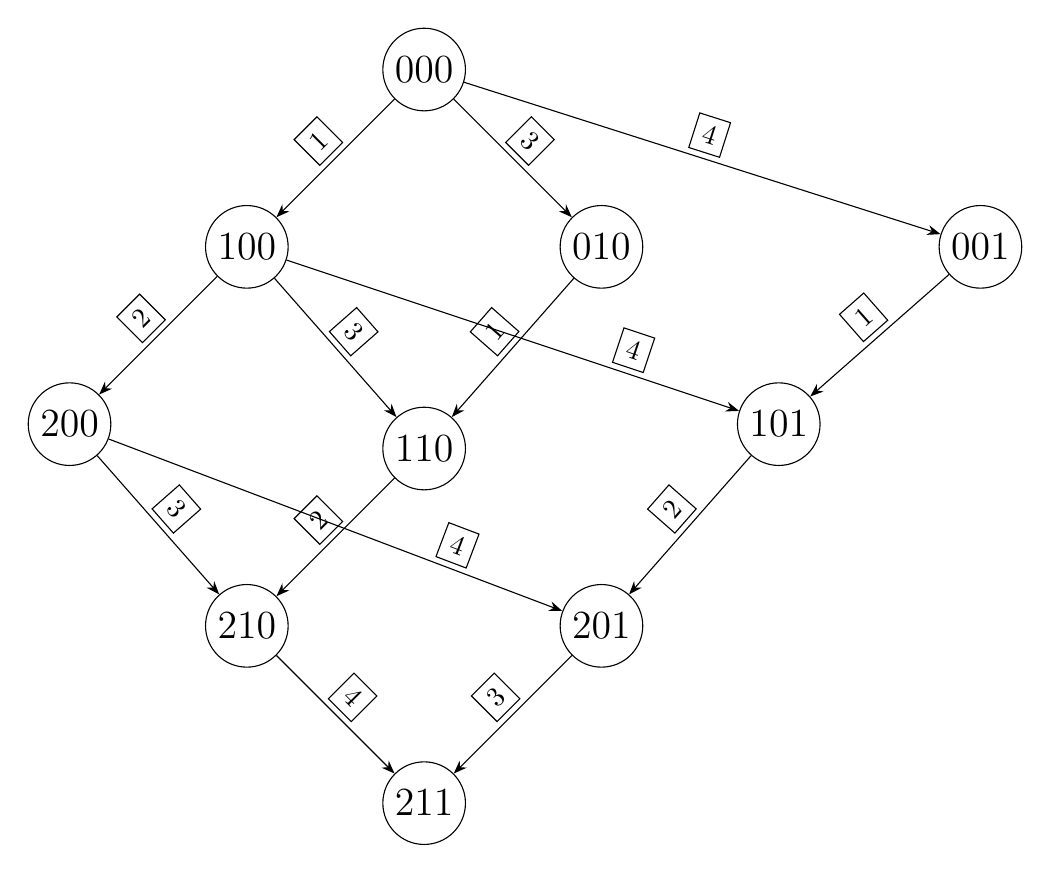
\begin{tikzpicture}
  \state{000}{}{(0,0,0)}

  \state{100}{below left = of 000}{(1,0,0)}
  \transition{000}{100}{1}

  \state{200}{below left = of 100}{(2,0,0)}
  \transition{100}{200}{2}

  \state{010}{below right = of 000}{(0,1,0)}
  \transition{000}{010}{3}
  \state{110}{below = 2.5*\vdist of 000}{(1,1,0)}
  \transition{100}{110}{3}
  \transition{010}{110}{1}
  \state{210}{below = 2.5*\vdist of 100}{(2,1,0)}
  \transition{200}{210}{3}
  \transition{110}{210}{2}

  \state{001}{right = 2.5*\hdist of 010}{(0,0,1)}
  \transition{000}{001}{4}
  \state{101}{below right = of 010}{(1,0,1)}
  \transition[near end]{100}{101}{4}
  \transition{001}{101}{1}
  \state{201}{below right = of 110}{(2,0,1)}
  \transition[near end]{200}{201}{4}
  \transition{101}{201}{2}
  \state{211}{below right = of 210}{(2,1,1)}
  \transition{210}{211}{4}
  \transition{201}{211}{3}

  % \state{1}{below left = of (0,0,0)}
  % \state{2}{below right = of (0,0,0)}
  % \state{12}{below = 2*\vdist of (0,0,0)}
  % \transition{0}{2}{2}
  % \transition{1}{12}{2}
  % \transition{2}{12}{1}
  % \state{3}{right = 1.5*\vdist of 2}
  % \transition{0}{3}{3}
  % \state{13}{right = 2*\hdist of 12}
  % \transition[near end]{1}{13}{3}
  % \transition{3}{13}{1}
  % 
  % \state{123}{below = 2*\vdist of 2}
  % \transition{12}{123}{3}
  % \transition{13}{123}{2}
\end{tikzpicture}
\end{document}